\section{Durchführung}
\label{sec:Durchfuehrung}

\subsection{Messung der Zeitkonstanten}
\label{sec:BestimmungderZeitkonstanten}
Es soll die Zeitkonstante des RC-Kreises bestimmt werden. Dazu wird die in Abbildung \ref{fig:Zeitkonstante} 
gezeigte Schaltung verwendet. Es wird ein Kondensator mit der Kapazität $C$ und ein Widerstand $R$ verwendet.
Weiterhin wird durch einen Spannungsgenerator eine Rechtecksspannung angelegt und
die Entladekurve kann durch das Oszillokop betrachtet werden.
\begin{figure}
    \centering
    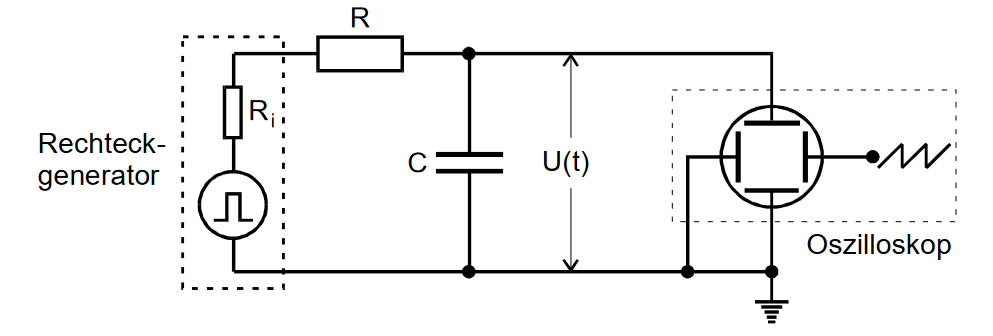
\includegraphics[width=0.7\textwidth]{Zeitkonstante.png}
    \caption{Schaltung zur Messung der Zeitkonstanten \cite{sample}.}
    \label{fig:Zeitkonstante}
\end{figure}

\subsection{Messung der Amplitude der Kondensatorspannung}
\label{sec:AmplitudeKondensatorspannung}
Bei dieser Messung bleibt der Versuchsaufbau unverändert. Es wird lediglich am Spannungsgenerator eine Sinusspannug
eingestellt. Die Frequenz $f$ der Spannung wird im Bereich von $\SI{250}{\hertz}$ bis $\SI{60}{\kilo\hertz}$
gemessen. Die Kondensatorspannungsamplitude $A$ kann wieder am Oszilloskop abgelesen werden.

\subsection{Messung der Phasenverschiebung}
\label{sec:Phasenverschiebung}
Nun wird die Schaltung zu der in Abbildung \ref{fig:SchaltungPhasenverschiebung} gezeigten Schaltung
geändert. Das Oszilloskop zeigt nun die Spannungsverläufe des Kondensators $U_{C}(t)$ und des Generators
$U_{G}(t)$ an. Die Spannungsverläufe sind in Abbildung \ref{fig:Phasenverschiebung} skizziert. Dabei wird
der Abstand der Nullstellen $a$ gemessen und die Wellenlänge $b$ von $U_{G}(t)$. Der Messbereich ist der 
gleiche wie in Abschnitt \ref{sec:AmplitudeKondensatorspannung}.

\begin{figure}
    \centering
    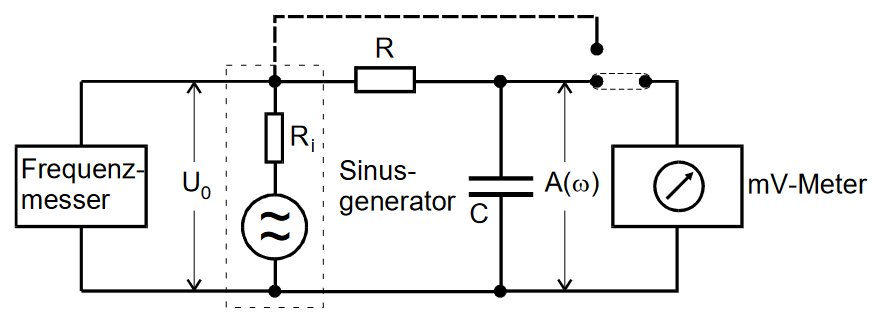
\includegraphics[width=0.7\textwidth]{Phasenverschiebung_Schaltkreis.png}
    \caption{Schaltung zur Messung der Phasenverschiebung \cite{sample}.}
    \label{fig:SchaltungPhasenverschiebung}
\end{figure}

\subsection{Messung zur Bestätigung der Integratorfunktion}
\label{sec:Integratorfunktion}

Nun wird die in Abbildung \ref{fig:Integrator} gezeigte Schaltung verwendet. Auf dem Zweikanal-Oszillographen 
ist nun die generierte Spannung und die integrierte Spannung zu sehen. Es werden jeweils Rechtsecks-, Sinus- und
Dreiecksspannung am Generator eingestellt und von jeder Einstellung ein Bild gemacht.

\begin{figure}
    \centering
    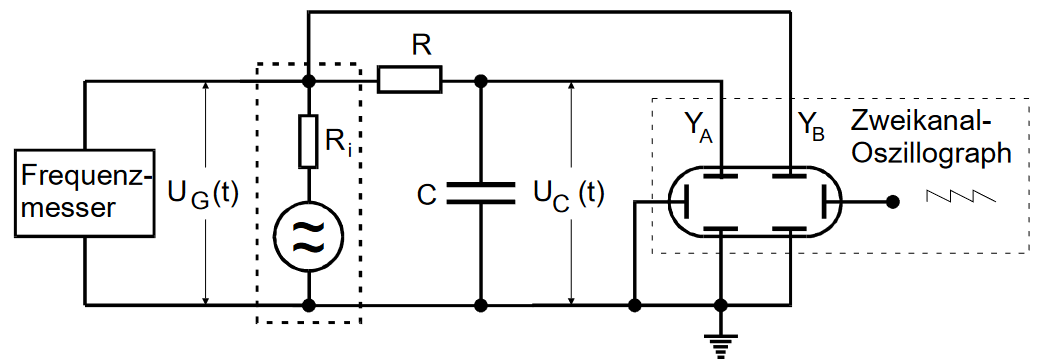
\includegraphics[width=0.7\textwidth]{Integrator.png}
    \caption{Schaltung zur Überprüfung des Integrators \cite{sample}.}
    \label{fig:Integrator}
\end{figure}
